\chapter{Design}
% 
\section{Domain Model}
\label{sec:Domain Model}
% 
\subsection{Domain Model Diagram}
\label{subsec:Domain Model Diagram}
\begin{figure}[H]
    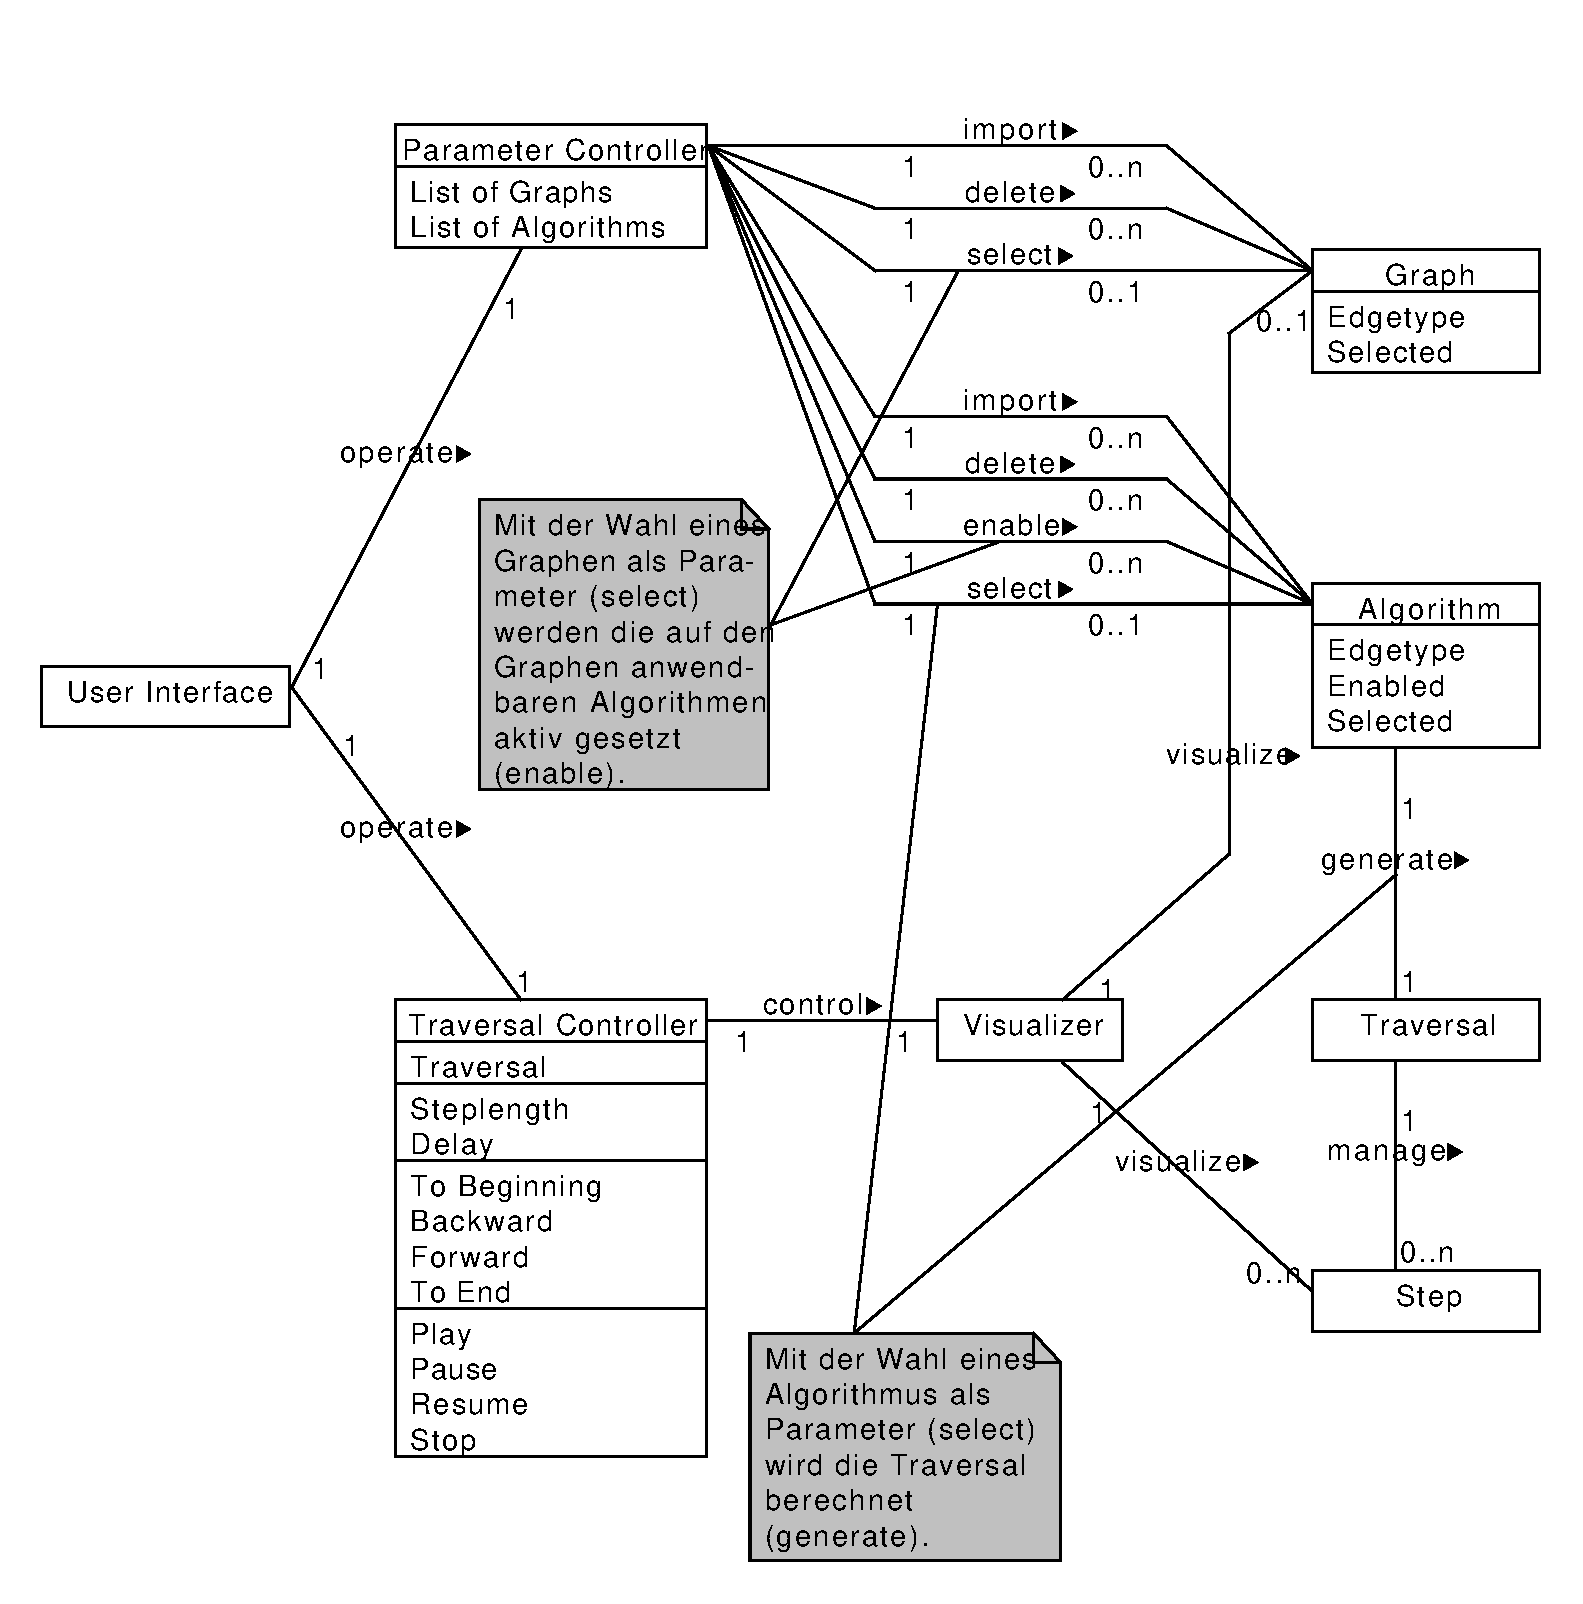
\includegraphics[totalheight=0.6\textheight]{diagrams/domain-model-diagram.pdf}
    \caption{Domain Model Diagram}
    \label{fig:domain_model_diagram}
\end{figure}
% 
\subsection{Domain Model Description}
\label{subsec:Domain Model Description}
Es folgt eine Beschreibung der Konzeptklassen (conceptual classes) mit Assoziationen, wie im Domain Model Diagram gezeigt. Multiplizit\"aten und Attribute werden in Klammern angegeben.
% 
\subsubsection{User Interface}
\label{subsubsec:User Interface}
\begin{itemize}
  \item \"Uber ein User Interface (1) kann ein User einen Parameter Controller (1) bedienen (\textit{operate}).
  \item \"Uber ein User Interface (1) kann ein User einen Traversal Controller (1) bedienen (\textit{operate}).
\end{itemize}
% 
\subsubsection{Parameter Controller}
\label{subsubsec:Parameter Controller}
\begin{itemize}
  \item Ein Parameter Controller verwaltet die zur Traversal ben\"otigten Parameter Graph (\textit{List of Graphs}) und Algorithm (\textit{List of Algorithms}).
  \item Der Parameter Controller h\"alt eine gegebene Anzahl von Graphen als Vorlagen bereit.
  \item Per Parameter Controller (1) kann ein User einen oder mehrere Graphen (0..n) des Formates *.graphml importieren (\textit{import}). Die importierten Graphen werden der Liste mit Graphen (\textit{List of Graphs}) hinzugef\"ugt.
  \item Per Parameter Controller (1) kann ein User vormals importierte Graphn (0..n) wieder l\"oschen (\textit{delete}). Diese werden aus der Liste mit Graphen (\textit{List of Graphs}) wieder entfernt.
  \item Per Parameter Controller (1) kann ein User einen Graphen (0..1) als Parameter ausw\"ahlen (\textit{select}).
  \item Mit der Wahl eines Graphen (1) als Parameter werden die auf den Graphen anwendbaren Algorithmen (0..n) aktiv gesetzt (\textit{enable}).
  \item Ein Parameter Controller h\"alt eine gegebene Anzahl Algorithmen als Vorlagen bereit.
  \item Per Parameter Controller (1) kann ein User einen oder mehrere Algorithmen (0..n) importieren (\textit{import}), sofern diese ein gefordertes Interface implementieren. Die importierten Algorithmen werden der Liste mit Algorithmen (\textit{List of Algorithms}) hinzugef\"ugt.
  \item Per Parameter Controller (1) kann ein User vormals importierte Algorithmen (0..n) wieder l\"oschen (\textit{delete}). Diese werden aus der Liste mit Algorithmen (\textit{List of Algorithms}) wieder entfernt.
  \item Per Parameter Controller (1) kann ein User einen aktivierten (\textit{Enabled}) Algorithmus (0..1) als Parameter ausw\"ahlen (\textit{select}).
\end{itemize}
% 
\subsubsection{Graph}
\label{subsubsec:Graph}
\begin{itemize}
  \item Ein Graph hat ungerichtete oder gerichtete Kanten (\textit{Edgetype}).
  \item Ein Graph kann ausgew\"ahlt werden (\textit{Selected}).
\end{itemize}
% 
\subsubsection{Algorithm}
\label{subsubsec:Algorithm}
\begin{itemize}
  \item Ein Algorithm kann Graphen mit ungerichteten oder gerichteten Kanten (\textit{Edgetype}) verarbeiten.
  \item Ein Algorithm (1) generiert eine Traversal (1) (\textit{generate}).
  \item Ein Algorithm kann aktiviert werden (\textit{Enabled}).
  \item Ein aktivierter Algorithm (\textit{Enabled}) kann ausgew\"ahlt werden (\textit{Selected}).
  \item Mit der Wahl eines Algorithm (1) als Parameter (\textit{Selected}) wird eine Traversal (1) erstellt (\textit{generate}).
\end{itemize}
% 
\subsubsection{Traversal}
\label{subsubsec:Traversal}
\begin{itemize}
  \item Die Traversierung ist ein visualisierbares Objekt.
  \item Eine Traversal (1) kann einen oder mehrere Steps (0..n) verwalten (\textit{manage}).
\end{itemize}

\subsubsection{Step}
\label{subsubsec:Step}
\begin{itemize}
  \item Ein Step ist ein Schritt der Traversierung.
\end{itemize}

\subsubsection{Traversal Controller}
\label{subsubsec:Traversal Controller}
\begin{itemize}
  \item Ein Traversal Controller (1) steuert einen Visualizer (1) (\textit{control}).
  \item Der Traversal Controller h\"alt eine Traversierung (\textit{Traversal}).
  \item Per Traversal Controller kann ein User die Anzahl Schritte pro Bild (\textit{Steplength}) einstellen.
  \item Per Traversal Controller kann ein User die Zeit zwischen zwei Bildern (\textit{Delay}) einstellen.
  \item Per Traversal Controller kann ein User Step-by-Step-Elemente (\textit{Forward, Backward, To Beginning, To End}) bedienen.
  \item Per Traversal Controller kann ein User Animations-Elemente (\textit{Play, Pause, Resume, Stop}) bedienen.
\end{itemize}

\subsubsection{Visualizer}
\label{subsubsec:Visualizer}
\begin{itemize}
  \item Ein Visualizer (1) kann einen Graphen (0..1) visualisieren (\textit{visualize}).
  \item Ein Visualizer (1) kann einen oder mehrere Steps (0..n) visualisieren (\textit{visualize}).
\end{itemize}